\subsubsection{Event Variables}
\bcool enables the definition of new events by using \emph{Event variables}. Such events can be either defined globally for the whole specification (\emph{globalEventVariables}) or locally within the operator (\emph{localEventVariables}). To illustrate the use of event variables, we slightly modify the example presented in Listing~\ref{lst:bcoolrunningexample2}. We consider the case where the synchronization of FSMEvents and Actions is based on a global clock signal. This situation is frequent in synchronous digital systems where a clock signal is used to coordinate actions within a circuit. As a result, the communication is forced to happen only when the global clock ticks. 

\begin{lstlisting}[language=bcool,
caption={Synchronized product operator between the TFSM and Activity languages by using Event Variables},
label={lst:bcoolrunningexample2}, 
basicstyle=\scriptsize\ttfamily, backgroundcolor=\color{LGrey}, numbers=left, xleftmargin=2pt]
BCOoLSpec TFSM-fUMLOperators
ImportLib "facilities.bcoollib"
ImportInterface "activitySemantics.ecl" as activity
ImportInterface "TFSM.ecl" as tfsm

Global Event globalClock;

Operator SyncProduct(dse1 : activity::startAction, dse2 : tfsm::occurs)
CorrespondenceMatching: when (dse1.name = dse2.name)
CoordinationRule: 
	Local Event sampledStartAction = Sample (globalClock, dse1);
	Local Event sampledOccurs = Sample (globalClock, dse2);
	
	RendezVous(sampledstartAction, sampledoccurs)
end operator
\end{lstlisting}

To specify a global clock, we define a global event variable named \emph{globalClock} (Listing~\ref{lst:bcoolrunningexample2}: line 6). This event variable can then be used across different operators as a synchronization variable. %In this example, we use \emph{globalClock} as a parameter to create two local variables named \emph{sampledOccurs} and \emph{sampledStartAction} (Listing~\ref{lst:bcoolrunningexample2}: line 11 and 12). 

The definition of event variables can be made by using an \emph{EventExpression} that returns a new event from a given parameter. For instance, this can be used to select only some occurrences of a \dse instance, thus allowing the implementation of filters. An event expression can also be used to join in a single event the occurrences of different events (union). 

\begin{figure}[h]
	\center
	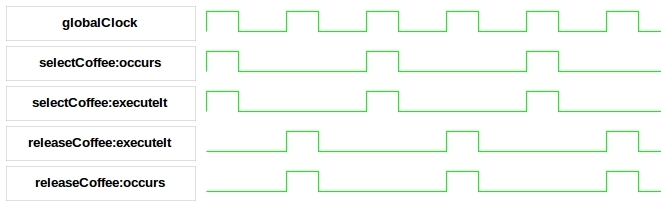
\includegraphics[width=.5\textwidth]{bcool/figs/runningeventvar}
	\caption{Resulting coordination of the Coffee Machine by using the Event Variables TODO: To show local event variables}
	\label{fig:runningeventvar}
\end{figure}

In our example, we rely on the event expression \emph{Sample} (see Appendix~\ref{ap:expressionandrelations}). Then, we use the globalClock and instances of \dse as parameters to create two local event variables (Listing~\ref{lst:bcoolrunningexample2}: line 11 and 12). The resulting events tick if and only if the global clock and the instance of \dse have also ticked. For instance, the event \emph{sampledOccurs} only ticks if globalClock and the instance of \dse \emph{occurs} ticks. In this case, we use a global event variable together with event expressions to sample the occurrences of selected instances of \dse. Then, we can use the local events as parameters of event relations, constraining by transitivity (some of) the occurrences of \dse instances. In our example, we force a simultaneous occurrence between the local events by using the relation rendezvous (Listing~\ref{lst:bcoolrunningexample2}: line 13). As a result, instances of \dse occurs and startAction happen simultaneously (see Figure~\ref{fig:runningeventvar}). 

\begin{lstlisting}[language=bcool,
caption={Synchronized product operator between the TFSM and Activity languages by using a Filter},
label={lst:bcoolrunningexample3}, 
basicstyle=\scriptsize\ttfamily, backgroundcolor=\color{LGrey}, numbers=left, firstnumber=10, xleftmargin=2pt]
CoordinationRule: 
	Local Event dividerFrec = Filter (globalClock, 4)
	Local Event sampledStartAction = Sample (dividedFrec, dse1);
	Local Event sampledOccurs = Sample (dividedFrec, dse2);

	RendezVous(sampledstartAction, sampledoccurs)
end operator
\end{lstlisting}

In the following example, we illustrate the use of Event variables by implementing a frequency divider. To do so, we use the event expression \emph{Filter} on the global clock. This results in a new event variable named \emph{dividerFrec} that ticks every four occurrences of the global clock (four is also a parameter). We modify the coordination rule of the previous example (see Listing~\ref{lst:bcoolrunningexample3}). We first define a new local event named \emph{dividerFrec} by using the event expression \emph{Filter} (see Appendix~\ref{ap:expressionandrelations}). The resulting event ticks every four occurrences of the globalClock (Listing~\ref{lst:bcoolrunningexample3}: line 11). We then replace the global clock by the dividerFrec clock (Listing~\ref{lst:bcoolrunningexample3}: line 12 and 13). Figure~\ref{fig:runningeventvarfilter} shows the resulting coordination where the synchronization between FSMEvents and Actions relies on the local event \emph{dividerFrec} that ticks every four occurrences of the global clock.  
 
\begin{figure}[h]
 	\center
 	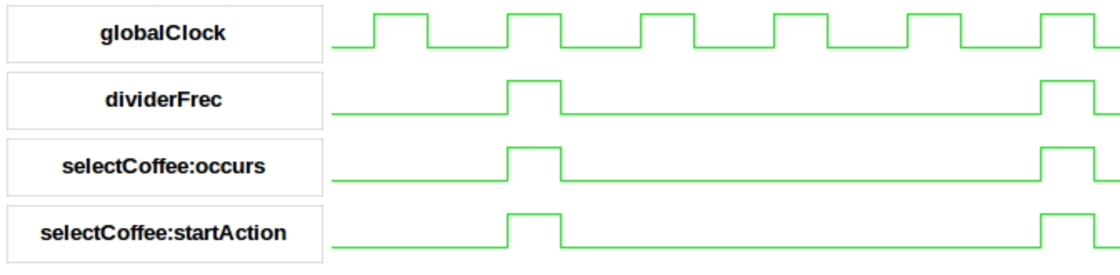
\includegraphics[width=.6\textwidth]{bcool/figs/runningeventvarfilter}
 	\caption{Resulting coordination of the Coffee Machine by using the Event Variables TODO: To show local event variables}
 	\label{fig:runningeventvarfilter}
\end{figure}

\todo{Event expression are defined into dedicated libraries that must be imported (see Section~\ref{subsec:bcoollib}).}

\todo{To link to the next section libraries}